%Het eerste hoofdstuk van je thesis.
\chapter{Literatuurstudie}
De literatuurstudie schetst een beeld van de sateliet constellaties die gebruikt worden. Deze worden besproken in \ref{LGNS}. Eens we de verschillende types van satelieten kennen, besrpeken we de manier waarop ze met elkaar communiceren in sectie \ref{LCom}.

\section{GNSS}
\label{LGNS}
GNSS ofwel Global Navigation Satellite System, is een sateliet systeem met een wereldwijde dekking. GNSS is een standaard term gebruikt om systemen te beschrijven die positie en navigatie oplossingen bieden. Het werd voornamelijk ontwikkeld voor de luchtvaart en ruimtevaart industrie en militaire doeleinden. Tegenwoordig worden deze technologie\"en ook in andere toepassingen gebruikt. GNSS vraagt samenwerking tussen verschillende publieke en private organisaties \cite{LBibGNSS3}.  Dit systeem is opgebouwd uit verschillende subsystemen die verder in deze tekst bepsroken worden. Namelijk: GPS besproken in sectie \ref{LGPS}, In sectie \ref{LGLO} bespreken we GLONASS, Galileo wordt besproken in sectie \ref{LGal} en BeidDou komt al laatste aan bod in sectie \ref{LBeD}. Het IGS, International GNSS Service staat in voor de aflevering van de hoogste kwaltieit GNSS data en producten \cite{LBibGNSS}. Elke satelliet is een project op zichzelf. Hierdoor is het moeilijk om een gestandaardiseerde productie ketting te creëren \cite{LBibGNSS3}. Om de performantie van GNSS te meten zijn beschikbaarheid, betrouwbaarheid en nauwkeurigheid sleutel parameters. Met de beschikbaarheid bedoelt men het aantal satellieten dat zichtbaar is vanaf de positie van de gebruiker. De nauwkeurigheid is een maat voor hoe dicht de navigatie oplossing die door het systeem voorzien wordt is bij de echte locatie en snelheid van de gebruiker \cite{LBibGNSS6}.

\subsection{GPS}
\label{LGPS} 
GPS staat voor Global Positioning System. Dit is het satelieten gebaseerde positie systeem dat bij ons het bekendste is. Het is ontwikkeld in Amerika \cite{LBibGNSS}\cite{LBibGNSS3}. het is \'e\'en van de langst gebruikte systemen binnen GNSS en draait momenteel op volledige capaciteit \cite{LBibGNSS4}. Voor de gebruikers is kost van de data een hoge bezorgdheid. Daarom is het belangrijk om de kosten van de operaties te verkleinen. GPS moet toegankelijk zijn voor meerdere clients. De gebruikerstoegang gebeurt voornamelijk door mobiele toestellen die verbindig maken via het internet \cite{LBibGPS}. Voor sommige toepassingen voldoen de nauwkeurigheid en de betrouwbaarheid van de GPS constellatie niet \cite{LBibGNSS6}.

\subsubsection{Opbouw constellatie}
 De constellatie van GPS bestaat uit 32 satellieten en heeft zijn volledgie functionele capaciteit bereikt (FOC), het systeem wordt geleidelijk aan gemoderniseerd \cite{LBibGNSS4}. De satellieten zijn geplaatst in een bijna circulaire baan met een straal van 2562.75km. De periode bedraagt 11 uur en 58 minuten. Dit is de tijd die verstrijkt tussen dat een satelliet terug op dezelfde plaats wordt waargenomen. De satellieten worden geplaatst in 6 orbitale vlakken. De vlakken zijn gelijk geplaatste in de lengte richting. Maar de satellieten in elk vlak zijn niet op gelijke afstand geplaatst \cite{LBibGNSS6}. 

\subsubsection{Signalen}
Het GPS signaal bestaat uit twee zeer stabiele, bijna monochromatische draaggolven L1 en L2, waarop drie modulaties op aanwezig zijn:
\begin{itemize}
	\item C/A code
	\item P code
	\item broadcast bericht
\end{itemize}. 
Alle componenten van een GPS signaal zijn gebaseers op een fundamentele kloksnelheid f\textsubscript{0} van 10,23 MHz. De GPS draaggolven hebben een frequentie van 154 f\textsubscript{0} voor L1 en een frequentie van 120 f\textsubscript{0} voor L2\cite{LBibGPS2}. GPS signalen zijn modulaties van de draaggolven L1 en L2 voor alle satellieten \cite{LBibGPS3}.

\subsubsection{Manieren om posities te bepalen}
\paragraph{Differential GPS Corrections}
Differential GPS Corrections ook weel DGPS genoemd, worden gebruikt om nauwkeurig posities  te bepalen. Er worden minimaal twee GPS ontvangers gebruikt. Van \'e\'en van deze ontvangers moet de preciese postie gekend zijn, dit noemen we de basis ontvanger \cite{LBibGNSS2,LBibRTK}. De basis ontvanger gaat data verzenden over een radio link.  Het tweede station kan in bewging zijn, dit is echter geen voorwaarde. Het tweede station berekend zijn positie aan de hand van de data hij ontvangt van de satellieten maar ook van de data die het krijgt via de radio link van het basis station \cite{LBibRTK}. Dit is een populaire manier om sateliet en klok fouten te elimineren. Een nadeel van deze techniek is dat de observaties van beide stations simultaan moeten gebeuren \cite{LBibGNSS2}. Deze techniek geeft meedstal een resultaat op 1m nauwkeurig \cite{LBibRTK}.

\paragraph{Real-Time Kinematic}
Real-Time Kinematic wordt vaak afgekort als RTK. RTK is een speciale vorm van DGPS dat ongever op centimeter nauwkerigheid werkt. Indien je door gebruik te maken van dit algoritme de positie wilt bepalen, moeten er minimaal vijf satellieten zichtbaar zijn. Anders werkt het niet of even traag als DPGS in vele toepassingen \cite{LBibRTK}. 

\paragraph{Precise Point Positioning}
of PPP is een techniek die werkt met \'e\'en ontvanger en is zeer effici\"ent. \cite{LBibGNSS4}

\subsection{GLONASS}
\label{LGLO}
GLONASS is \'e\'en van de langst gebruikte systemen binnen GNSS. Het is ontwikkeld door Rusland \cite{LBibGLONASS2}. GLONASS is een afkorting, het staat voor GLObal NAvigation Satelite System \cite{LBibBeiDou}.Het GLONASS systeem is opgebouwd uit vier elementen:
\begin{itemize}
	\item Orbitale constellatie van GLONASS satellieten
	\item Controle segment op de grond
	\item Racket/ruimte complex
	\item Gebruikers
\end{itemize} \cite{LBibGLONASS2} Het systeem wordt continu gemoderniseerd \cite{LBibGNSS4}. GLONASS-M satellieten vormen een tweede genereatie van satellieten die gebruikt worden. Deze tweede generatie heeft volgende voordelen:
\begin{itemize}
	\item Langere gegarandeerde levenstijd (zeven jaar in plaats van drie)
	\item Maakt gebruik van L2 signalen
	\item Stabielere klok
	\item Extra beschikbare navigatie data (zoals betere integritetiscontrole, informatie over absolute tijd beschikbaarheid van de satelliet nummer)
	\item inter-satellite radio link
	\item Betere zonnenpanelen postionering
	\item Lager niveau van onvoorspelde versnellingen
\end{itemize}
Door deze tweede generatie GLONASS-M satellieten zijn er nieuwe mogelijkheden voor satelliet navigatie. GLONASS is een betrouwbaar systeem, voornamelijk voor Real-Time Kinematic (RTK) mode in omgevingen met slechte zichtbaarheid \cite{LBibGLONASS}. Voor de werking van het navigatie satelliet systeem is het belangrijk dat alle plrocessen die plaats vinden tijdens de werking gesynchroniseerd zijn. GLONASS-K satelieten vormen de derde generatie. De grootste veranderingen ten opzichte van GLONASS M zijn:
\begin{itemize}
	\item Het gebruik van een derde frequentie om betrouwbarheid en nauwkeurigheid voor gebruikersnavigatie te vergroten.
	\item De levensduur van de satelliet is vergroot tot 10 jaar
	\item Het gewicht van de satelliet is gehalveerd
\end{itemize}\cite{LBibGLONASS2}.

\subsubsection{Opbouw constellatie} 
De constellatie is opgebouwd uit 24 satelieten \cite{LBibGNSS4}. Deze satelliten zijn geplaatst in drie orbitale vlakken met een onderlinge afstand van 120 graden \cite{LBibGLONASS2,LBibGNSS6}. Per vlak zijn er acht saellieten geplaatst. De periode per satelliet voor \'e\'en omwentelling rond de aarde is 11 uur en 15 minuten \cite{LBibGNSS6}.  Het systeem heeft zijn FOC bereikt in januari 1996 \cite{LBibGLONASS}. Het systeem is volledig gerevialiseerd en is volledig operationeel \cite{LBibGNSS4}.

\subsubsection{Signalen}
Terwijl bij GPS de signalen mudolaties zijn van de draaggolven L1 en L2 voor alle satellieten, zijn bij GLONASS de draag frequenties afhankelijk van het uitzendende kanaal. Er zijn 12 kanalen voor 24 satellieten \cite{LBibGPS3}.  
 
\subsection{Galileo}
\label{LGal}
Galileo is het Europees systeem \cite{LBibGNSS3}\cite{LBibGNSS4}. Het doel van Galileo is het aanbieden van een flexibelere en nauwkeurige postionerings service \cite{LBibGNSS4}. Galileo is ontworpen om Europa te voorzien van dezelfde GNSS capaciteit als dat van GPS \cite{LBibGNSS6}. De architectuur van Galileo specificeert een globaal integriteits concept. Dit wilt zeggen dat de nauwkeurigheid en de integriteit van de werking altijd wereldwijd bereikt moet worden en binnen de drempelwaarden moet blijven \cite{LBibGalileo}.  Het Galileo systeem voorziet verschillende gebruikers diensten. E\'en van deze diensten is de Safety of Life service, dit is een groot voordeel van Galileo  on vergelijking met GPS. In geval van een systeem fout moet de gebruiker binnen de zes seconden gewaarschuwd worden \cite{LBibGalileo}. 

\subsubsection{Opbouw constellatie}
De volledige constellatie zal bestaan  uit 30 satelieten in drie orbitale vlakken. Het systeem is momenteel nog onder contructie \cite{LBibGNSS4}. De satellieten zijn geplaatst op drie orbitale vlakken. De periode van een tocht om de aarde is 14 uur en 21 minuten. Er zijn 10 satellieten per vlak \cite{LBibGNSS6}. 
 
\subsection{BeiDou}
\label{LBeD}
Bei Dou is het satilieten systeem binnen GNSS dat ontwikkeld is in China. Het systeem wordt vaak  aangeduid met de afkorting BDS \cite{LBibBeiDou} Het voorziet PNT (Postioning, Navia gtion and Timing) services in de Aziatisch-Pacifische regio. Momenteel is BDS  beshikbaar voor regionale diensten. Eveneens in 2020 zullen BDS signalen beschikbaar worden voor wereldwijde gebruikers. Ondertussen worden er steeds meer stations uitgebreid met BDS ontvangers voor hoog-precisie GNSS toepassingen \cite{LBibBeiDou}.

\subsubsection{Opbouw constellatie}
De volledige constellatie telt 35 satellieten. Het zal volledig zijn tegen het einde van 2020 \cite{LBibGNSS4}.

\subsection{Besluit}
Eens de vier systemen volledig ingezet zijn, zijn er meer dan 100 satelieten beschikbaar voor nauwkeurige PNT toepassingen. Door het opkomen van de twee nieuwere systemen Galileo \ref{LGal} en BeiDou \ref{LBeD} en de het voortdurend moderniseren van GPS \ref{LGPS} en GLONASS \ref{LGLO} is de wereld van sateliet navigatie onderheving aan veranderingen \cite{LBibGNSS4}.Momenteel loopt er een Mutli-GNSS expirment (MGEX) dat data verzamelt van GPS?GLONASS, Galileo en BeiDou. De samenvoeging van multi-GNSS vergroot het aantal satellieten en bijgevolg wordt de geometrische observatie geoptimaliseerd \cite{LBibGNSS5}. De multiple-GNSS observaties met meerdere frequenties voorzien de onderzoekers van meerdere kansen om de Aardse ionosferische variaties en gedragingen te onderzoeken. GNSS observaties kunnen gebruikt worden om ionosferische traagheids correcties en gerelateerd atenschappelijk onderzoek \cite{LBibBeiDou}.

\section{Communicatie}
\label{LCom}
\subsection{EUREF Permanent Netwerk}
Het EUREF Permanent GNSS Network wordt ook wel EPN genoemd \cite{LBibEPN3,LBibEPN2,LBibEPN}. Het netwerk is gebaseerd op een relatie tussen site opperatoren van permanenten GNSS sites, die bereid zijn om hun data met het publiek te delen. Het EPN werkt nauw samen met het IGS \cite{LBibEPN3}. Het netwerk is opgebouwd uit 220 permanenten GPS stations waarvan er 29 ook GLONASS satellieten volgend. Het primaire doel van EPN is het European Terrestrial Reference Systems (ETRS89) onderhouden, dit gebeurt door de leden op vrijwillige basis. \cite{LBibEPN}  \cite{LBibEPN2}. Een ander doel is het beschikbaar stellen van GNSS data en preciese co\"ordinaten van GNSS stations beschikbaar stellen aan het publiek. Nieuwe stations worden aan het netwerk toegevoegd zodra ze voldoen aan alle vereisten. HEt EPN werkt met drie datacenters die gedefinieerd worden als regionale datacenters (RDC). Het Federal Agency for Cartography and Geodesy van Duitsland (BKG) en het Austrian Academy of Sciences (OLG)  datacenters, zijn verantwoordelijk voor de dagelijkse zaken. Alle EPN stations gaaan op vooraf gedefinieerde wegen hun data op regelamtige basis doorsturen naar het BKG en OLG \cite{LBibEPN2}. Het datacenter van Royal Observatory of Belgium (ROB) doet dienst als datacenter van het centrale bureau van het EPN. Dit datacenter is verantwoordelijk voor het hosten van alle historische EPN RINEX data met gecorrigeerde meta-data en 1 regionale broadcaster. \cite{LBibEPN2,LBibEPN3}. Het co\"ordineren van tijd analyse is eveneens een doel van het EPN. Dit om het EPN te versterken als geodetisch referentie netwerk. Van de nieuw ge\"installeerde antennes is 90 procent een multi-GNSS antenne. Hiervan is 75 procent ontworpen om GNSS en GLONASS te obeserveren, 25 procent is bovendien ook klaar om Galileo te ontvangen. Het netwerk is dus continu onder constructie. \cite{LBibEPN3}.

\subsection{RINEX data formaat}

\subsection{RTCM}
RTCM staat voor Radio Technical Commission for Maritime Services \cite{LBibGLONASS}.

\subsection{NTRIP}
\label{LNTR}
Networked Transport of RTCM via Internet Protocol of kortweg NTRIP \cite{LBibNTRIP,LBibNTRIP3}. NTTRIP is een protocol ontwikkeld in 2004 \cite{LBibNTRIP3}. Men maakt gebruik vant internet om de realtime GNSS data uit te wisselen en te verzamelen. NTRIP is een HTTP(Hypertext Transfer Protocol) stateless applicatie level protocol om GNSS te streamen over het internet \cite{LBibNTRIP}. De toepassing die men in gedachte had bij het ontwerpen van het protocol is het doorsturen van RTCM data, maar het protocol kan gebruikt worden om GNSS data in eender welk formaat door te sturen. De enige beperking is een maximum snelheid van 10 kb/s en een minimum van 100b/s \cite{LBibNTRIP3}. Deze techniek is ontwikkeld binnen het framwerk van EUREF. Het odeil is om real-time data uit te wisselen, maar ook om afgeleide producten te broadcasten, voornamelijk DGPS \cite{LBibNTRIP2}. De nodige brandbreedte hiervoor is niet groot in vergelijking met bijvoorbeeld Internet Radio\cite{LBibNTRIP}. Hierdoor wordt de NTRIP techniek een alternatief voor het verzenden van DGPS data tegenover andere  wereldwijde broadcasting technieken. Het internet is uitermate goed geschikt om data door te sturen tussen verschillende providers over een grote afstand \cite{LBibNTRIP2}. Het is gebaseerd op software die oorspronkelijk bedoelt was voor MP3 media speler formaten. Dit blijk wel aangepast te zijn voor GNSS stromen met data snelheden toosen 0.5 en 5 kbit/s. \cite{LBibGPS}. Een ander voordeel is dat tegenwoordig op veel plaatsen internet verbinding voorzien is \cite{LBibNTRIP}. Verder is er ook geen vermindering van de positie voorstelling door gebruik te maken van NTRIP. Een ander groot voordeel is dat datastromen van referentie stations simultaan beschikbaar worden via \'e\'en communicatie techniek. Men moet er wel rekening mee houden dat de nodige servers moeten verbonen worden aan het internet via intergeconnecteerde broadcasters met een voldoende grote bandbreedte.  De generatie van DPGS correctie data wordt meestal direct op de GPS ontvanger gedaa, maar hij kan eveneens bepaald worden van observaties die verkregen worden dooe verschillende referentie stations in het netwerk. De datastroom wordt dan door gegeven aan een server die de stroom vervolgens beschikbaar stelt over her internet via een geschikt protocol \cite{LBibNTRIP2}. Het gevolgde pad van de data wordt weergegeven in figuur \ref{imgNTRIP2}.
\begin{figure}[hpb]
	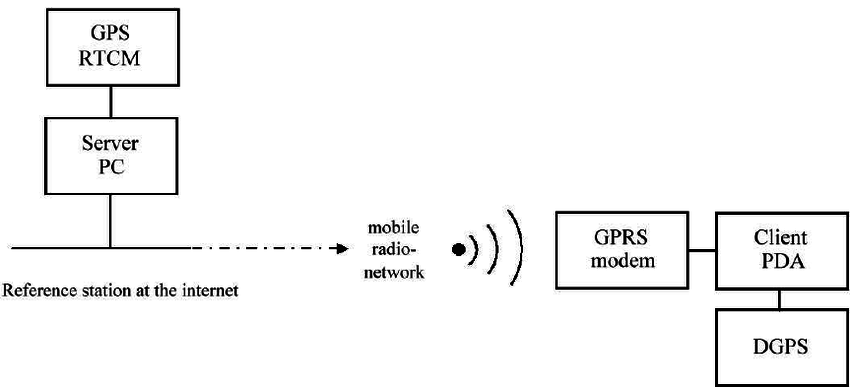
\includegraphics[scale=0.4]{NTRIP2.png}
	\caption{RTCM data stroom op het internet \cite{LBibNTRIP2}}
	\label{imgNTRIP2}
\end{figure} 
De afstand tussen het referentie staion en de client met het verbonden station is opgedeeld in twee delen. Het groote deel van de afstand bestaat uit een bedrade internet verbinding. Het overige deel wordt overbrugd door mobiele telefonie tehnologie \cite{LBibNTRIP2}.

\subsubsection{opbouw van NTRIP software}
\label{LONS}
NTRIP wordt ge\"implemeneteerd in vier grote componenten. Nameijk NTRIP Sources, Ntrip clients, NtripServers en NtripCasters. De NTRIP Sources stellen de bronnen van de GNSS data voor. Deze worde ngevoed aan het systeem/ Meestal is dit een GNSS ontvanger die obdervaties en voorziet of die DGPS correctie data genereert \cite{LBibNTRIP3}. De NtripCaster is het HTTP server programma terwijl NTRIPClients en NTRIPServers reageren zoals HTTP clients\cite{LBibNTRIP}. NTRIPServers gaat datastromen vervoeren. NTRIPCasters gaan de administratie tussen clients en servers afhandelen \cite{LBibGPS}. NTRIPCasters is een stream-spliteser en broadcaster component, momenteel zijn er acht NTRIPCasters in Europa \cite{LBibNTRIP}. De casters gaan zoals vaak gebeurt bij internet radio implementaties de binnenkomende datastromen dupliceren, zodat hij door meerdere gebuikers simultaan ontvangen kan worden \cite{LBibNTRIP2}.NTRIP omvat de voorziening van metadata door een Soaurce Table die onderhouden wordt door de NTRIP Caster \cite{LBibNTRIP3}.  NTRIP Clients gaan data ontvangen van de gewenste bronnen via de NTRIPCaster. NTRIPServers gaan de data van \'e\'en of meerdere bronnen verzenden in NTRIP formaat. Als laatste hebben we ook nog NTRPSorurces, deze genereren DPGS datastreams op een specifieke locatie \cite{LBibNTRIP}. In figuur \ref{imgNTRIP} staat een overzicht van de opbouw van het NTRIP streaming systeem. NTRIP is gebaseerd op een subset van het  vaak gebruikte HTTP an is bijgevolg dus gebaseerd op TCP. Daaruit volgt dat het streamen gebeurt vanuit een enkele IP Poort. MEestal is dit poort 80 of 2101 \cite{LBibNTRIP3}. 

\begin{figure}[hpb]
	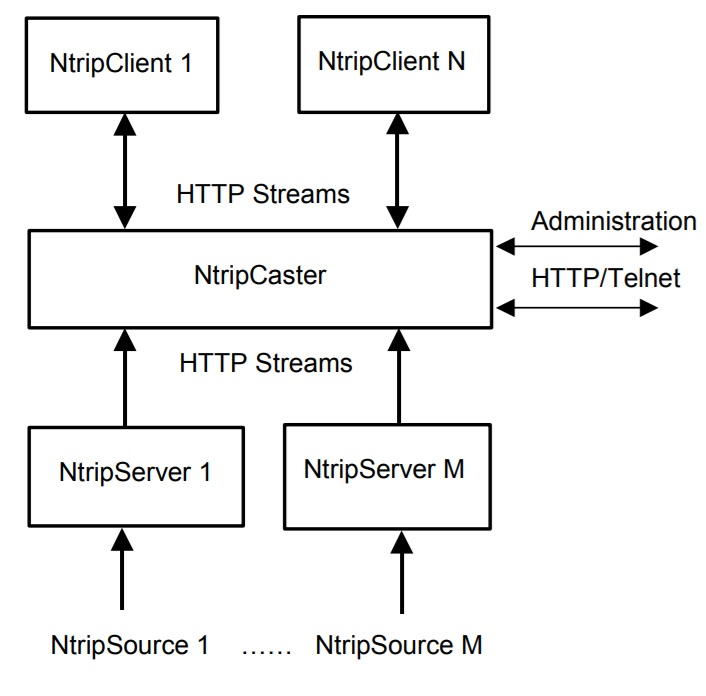
\includegraphics[scale=0.65]{NTRIP.jpg}
	\caption{NTRIP streaming systeem \cite{LBibNTRIP}}
	\label{imgNTRIP}
\end{figure} 
 



